\documentclass[varwidth=true, border=2pt]{standalone}
\usepackage{tkz-euclide}

\begin{document}
\usetkzobj{all}
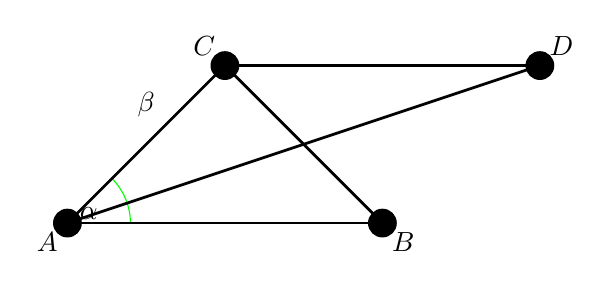
\begin{tikzpicture}
    \tkzSetUpPoint[shape=circle,size=10,color=black,fill=black]
    \tkzSetUpLine[line width=1]
    \tkzDefPoints{0/0/A, 4/0/B, 2/2/C, 6/2/D}

    \tkzMarkAngle[arc=l,size=0.8cm,color=green,fill=green!20](B,A,C)
    \path[draw] ++(25:.3) node[rotate=0] {$\alpha$};
    \node at (1,1.5) {$\beta$};
    \tkzDrawSegments(A,B A,C A,D B,C C,D)
    \tkzDrawPoints(A,B,C,D)
    \tkzLabelPoint[below left](A){$A$}
    \tkzLabelPoint[below right](B){$B$}
    \tkzLabelPoint[above left](C){$C$}
    \tkzLabelPoint[above right](D){$D$}
\end{tikzpicture}
\end{document}
